\documentclass[12pt,a4paper,english,twocolumn,fleqn]{narms}

% packages needed
\usepackage{subfigure}
\usepackage{epsfig}
\usepackage{timesmt}

% add here more packages based on the document format
\usepackage[usenames,dvipsnames,svgnames]{xcolor}
\usepackage[numbers, sort&compress]{natbib}

\usepackage{babel}
\usepackage{graphicx}
\usepackage{bm}

\usepackage{amsmath}
\usepackage{amsfonts}
\usepackage{amssymb}

\usepackage{siunitx}
%\sisetup{mode=text,range-phrase = {\text{~to~}}}
\sisetup{
  range-phrase = {,}\ ,
  range-units  = brackets,
  open-bracket = [,
  close-bracket= ],
}

\usepackage[colorlinks=true]{hyperref} % Hyperlinks within and outside the document
% false: boxed links; true: colored links

\usepackage[utf8]{inputenc}
\usepackage[T1]{fontenc}
\usepackage{textcomp}
\usepackage{lmodern} % German related symbols

% setting math equation indent from left 0pts
\mathindent=0pt%

%%%%%%% Style for TABLES
% insert tabular command inside \tabletext{} this will produce tables in 10pts

\defcitealias{Octave}{GNU Octave}
\defcitealias{Inkscape}{Inkscape}

\newcommand{\jpi}[1]{{\color{Magenta} JPi: #1}}
\newcommand{\seb}[1]{{\color{Red} Seb: #1}}

\begin{document}
\title{Fast early flood warning systems exploiting catchment specific behavior}
\author{{S. Rusca} \\
{\aff{Swiss Federal Institute of Aquatic Science and Technology, Eawag, Dübendorf, Switzerland}} \\\\
{\authornext{J. P. Carbajal}}\\
{\aff{Swiss Federal Institute of Aquatic Science and Technology, Eawag, Dübendorf, Switzerland}}
} \maketitle


\section*{Abstract}

We present a catchment specific emulator based on non-linear shallow water equations to be used
for early flood warning system in real time.

\section{Introduction}

Floods due to heavy rain are among the most destructive events in hydrology and their frequency has incremented over the last decades.
Numerical models are useful tools to predict floods and trigger security measures or evacuations. However, the high computation demands of these models hinders their use in real time early warning systems.

Fine tuned shallow water based simulators are able to produce trustworthy flood predictions but are unusable as early warning systems due to their high computational cost.
Early warning systems should be capable of quickly providing a prediction of whether, based on current conditions and meteorological forecast, an occurring rain event will result in major flooding or not, and if yes within how much time.
Fast surrogate models based on detailed simulators can provide accurate results\footnote{Note that accuracy is task dependent} with speed-up factors of up to $10^6$~\citep[see][for an application in geophysical hazards]{Bayarri2015}.

In this work, we present the development of a surrogate model of a detailed simulator using \textit{FullSWOF\textunderscore2D-v.1.07.00}~\citep{fullswof} (non-linear shallow water equations).

\section{Methodology}

The general goal of our emulator is to take inputs related to a rain event and catchment situation, and predict the time it will take to observe a catchment discharge greater or equal to a predefined threshold discharged $Q_!$.
The threshold discharge is provided by a downstream region that is prone to flooding and the quantity of interest (QoI) is the time-to-threshold, $t_!$.

The emulator is built using two input parameters: rain intensity ($I$) and soil saturation ($\Delta\theta$).
Simulations were run using the simulator with different values of these parameters and response hydrographs of a $\SI{2}{\kilo\metre} \times \SI{2}{\kilo\metre}$ synthetic catchment were recorded.
A set of \num{50} simulations were run with saturations in the $[\numrange{0}{1}]$ interval
and rain intensities in \SIrange{10}{30}{\milli\metre\per\hour}.
Fig.~\ref{img:topography} shows the synthetic topography used.

\begin{figure}[htpb]
  \centering
  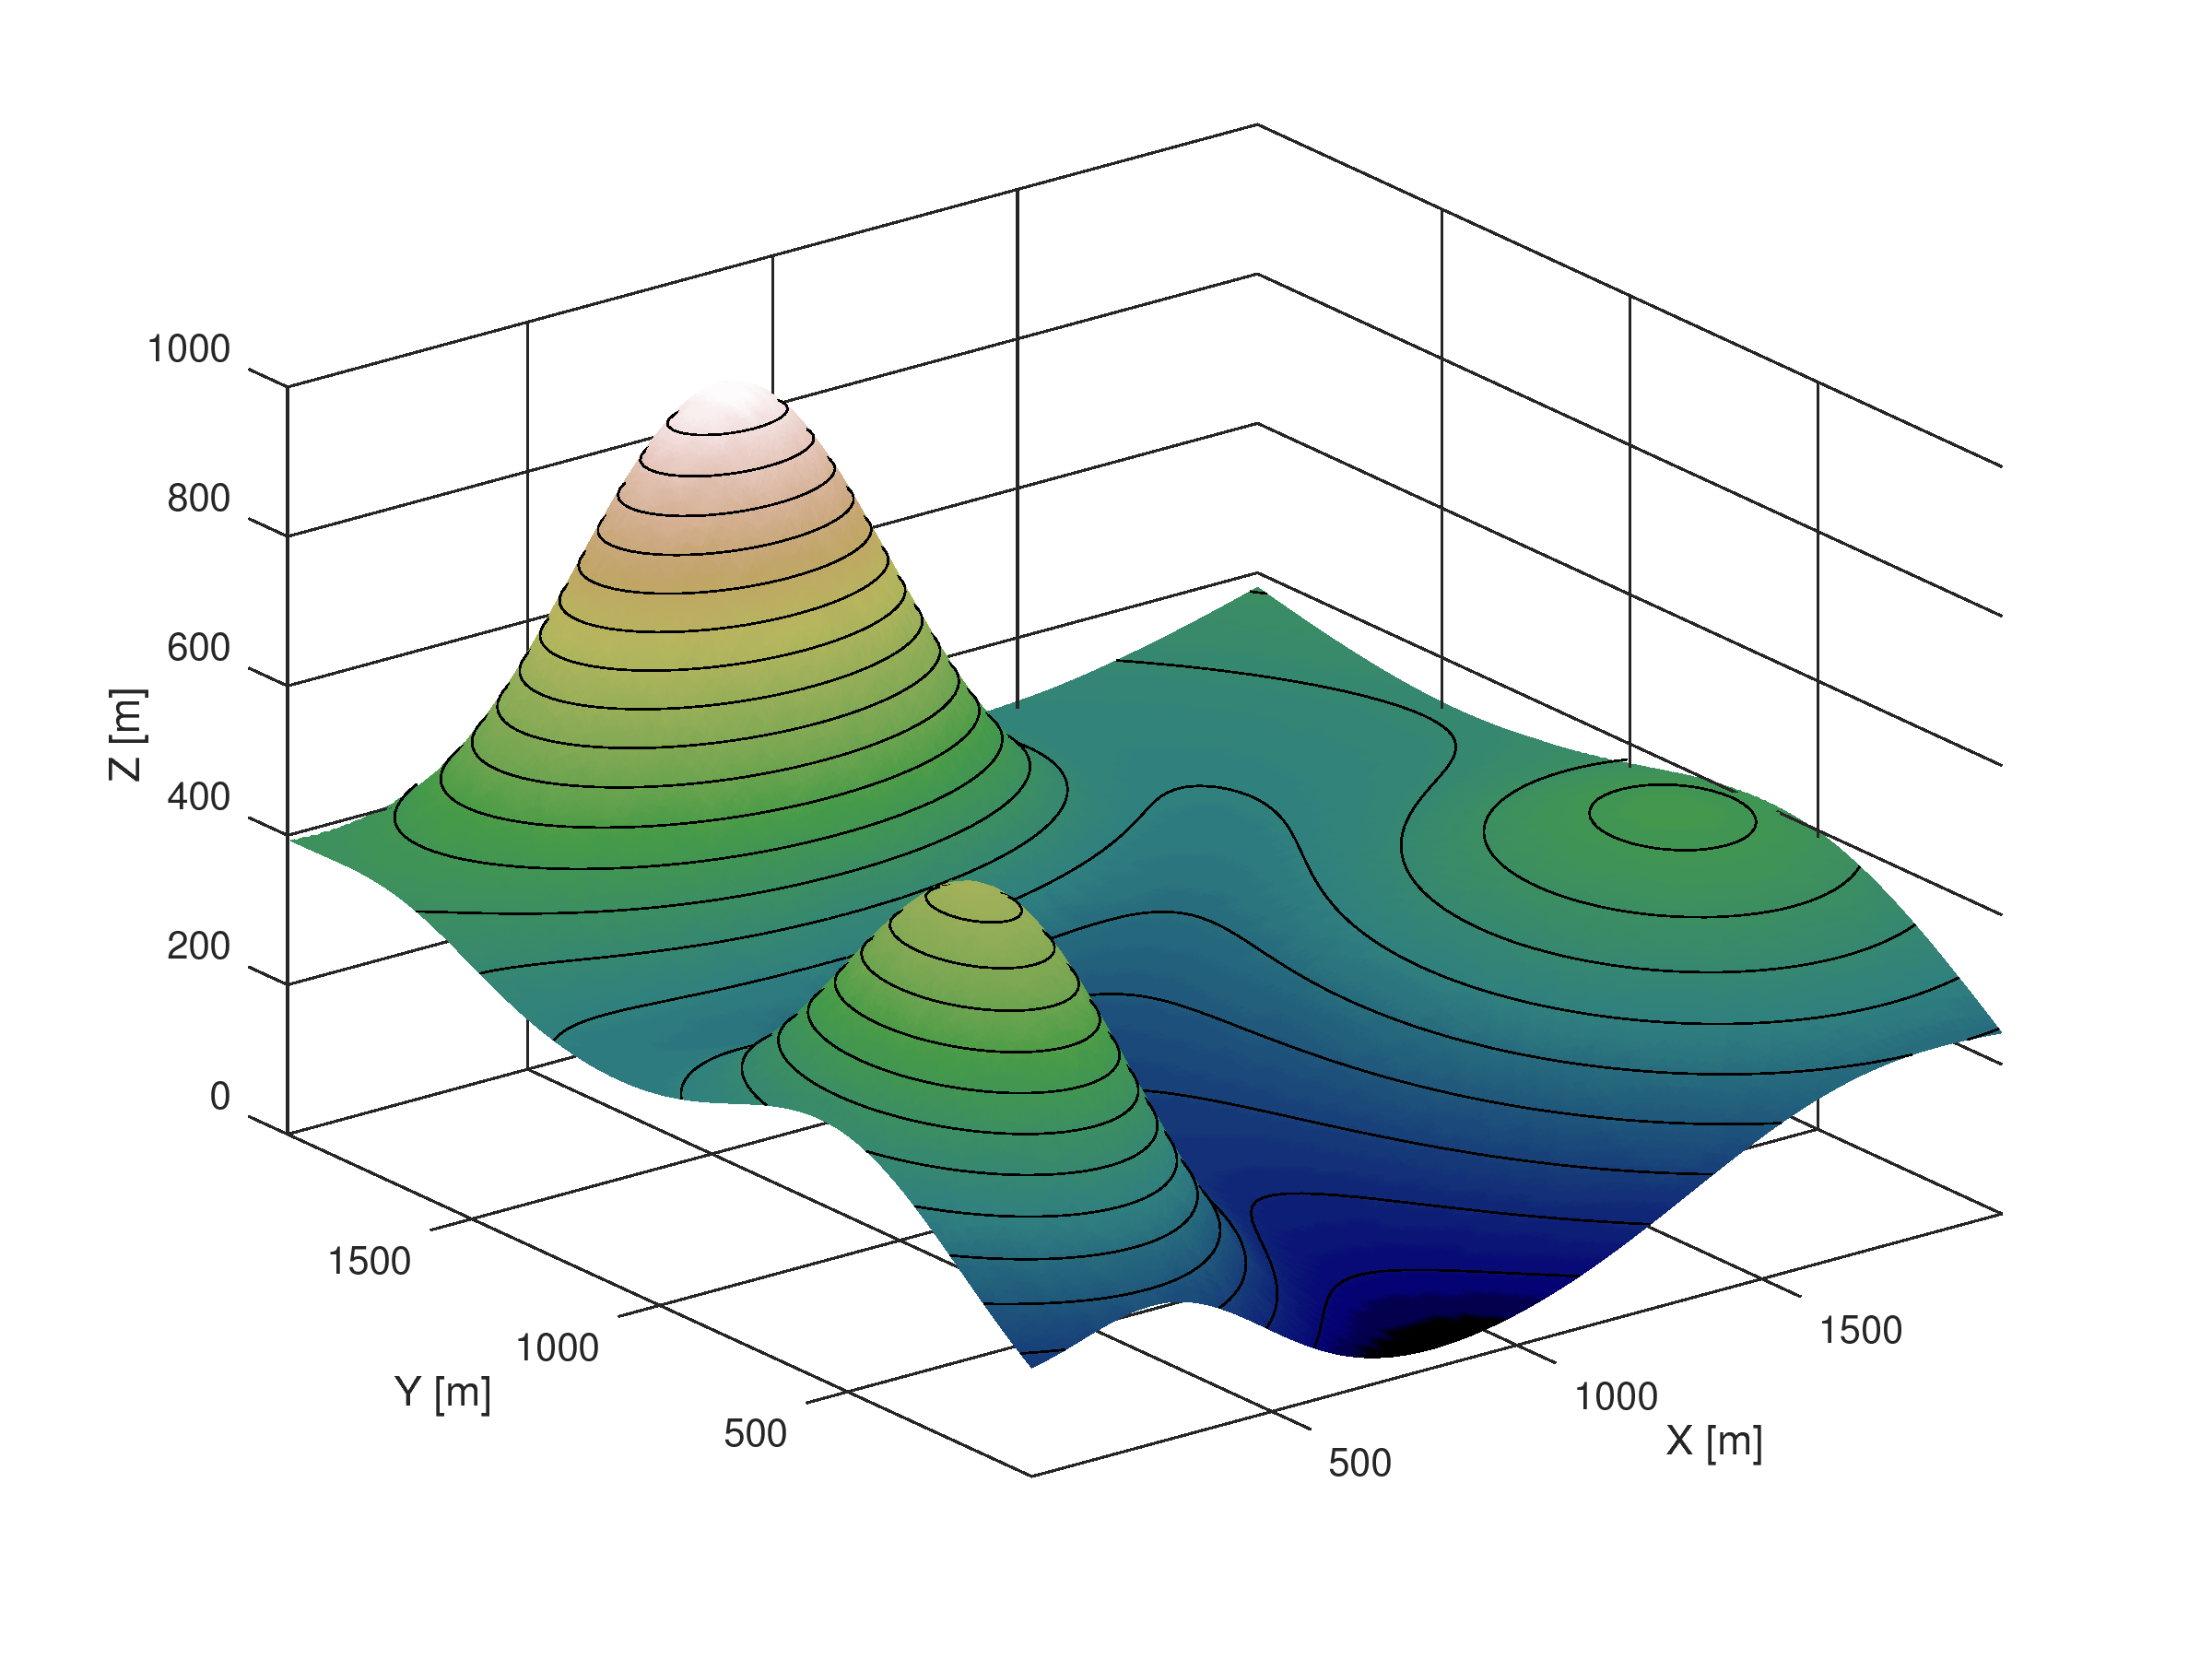
\includegraphics[width=0.4\textwidth]{img/topography.png}
  \caption{Synthetic topography defining a parabolic catchment with \num{3} Gaussian bumps.}
  \label{img:topography}
\end{figure}

The rationality behind the chosen parameters is that rain intensity is readily available from meteorological forecast, and soil saturation is used to incorporate the recent history of the catchment, e.g. if there were several rains in the previous days the soil will be highly saturated.

Since the response hydrograph shape is independent of rain duration, i.e. the effect of different rain durations can be factored out

\begin{equation}
Q(t, I, \Delta\theta, d) \approx Q_\infty(t, I, \Delta\theta) \Xi(t \leq d)
\end{equation}

\noindent where $Q$ is the response hydrograph, $t$ is the time variable, $d$ is the rain event duration, and $\Xi(x)$ is the indicator function of the interval $[\num{0},d]$.
This representation does not recover the recession of the hydrograph, but that is irrelevant for our application.
Fig.~\ref{img:hydrograph} shows an example response obtained from the simulator.
Recession of the discharge can be observed immediately after the end of the rain event.

\begin{figure}[htpb]
  \centering
  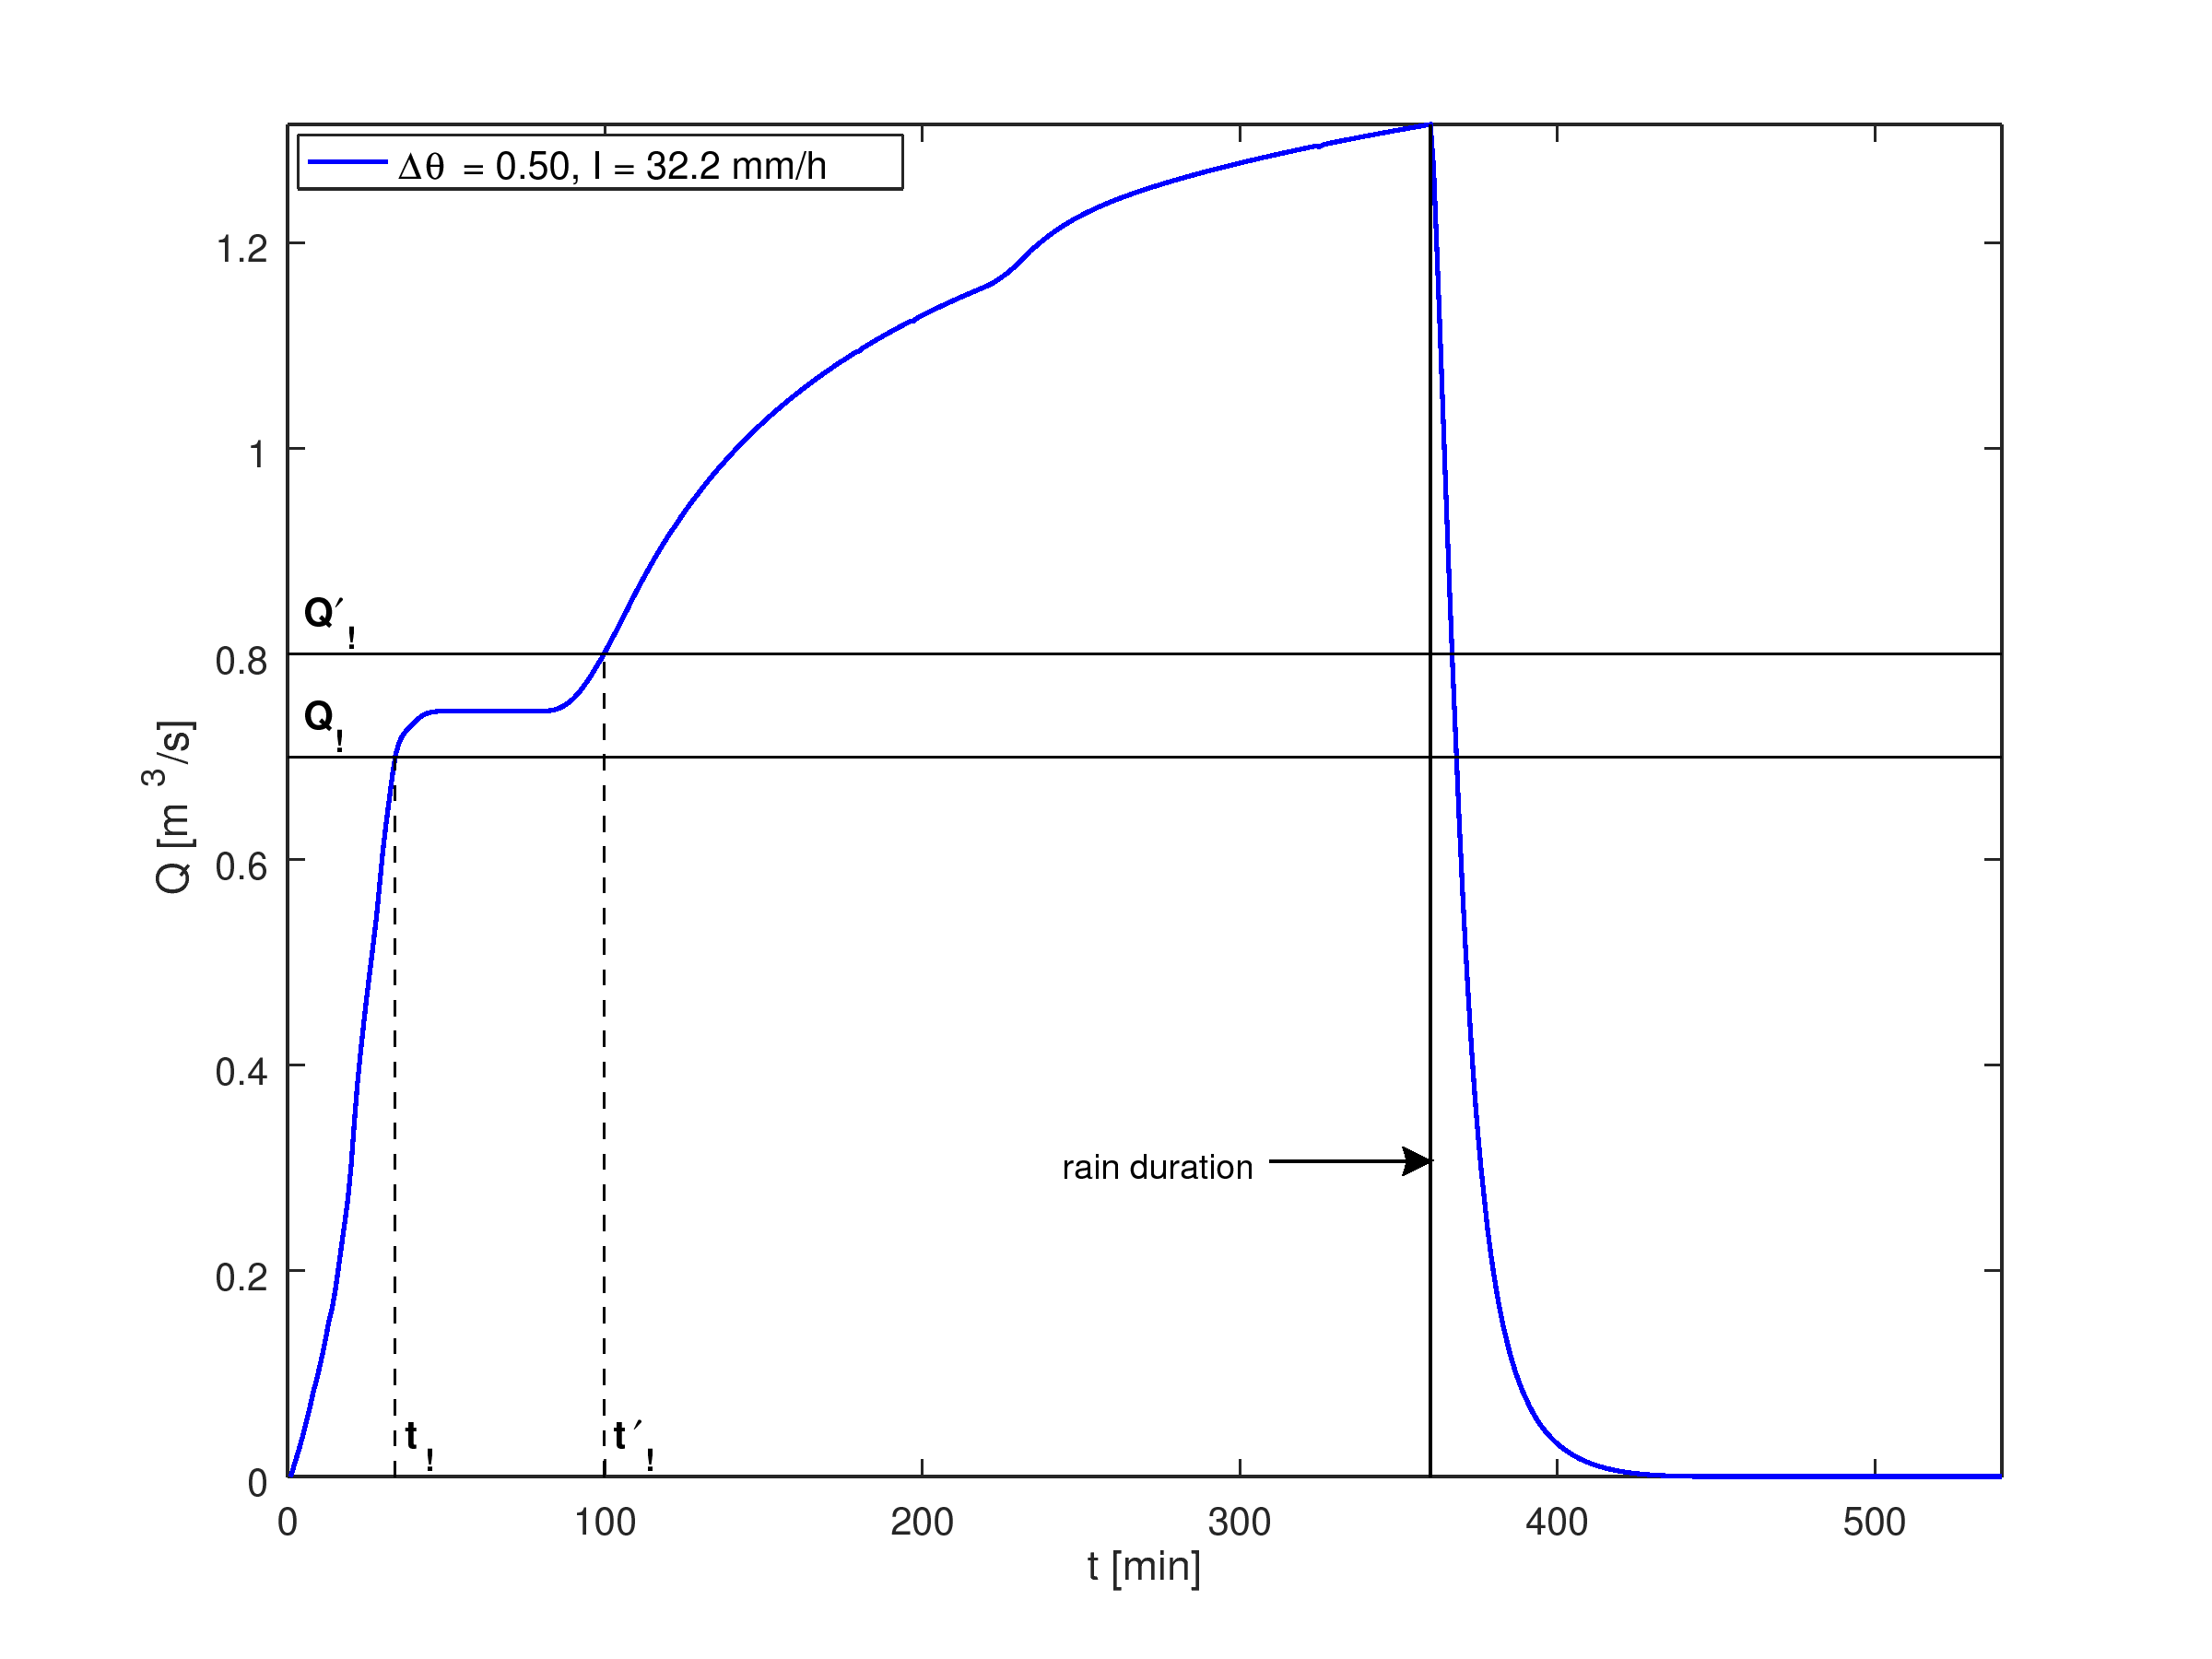
\includegraphics[width=0.4\textwidth]{img/hydrograph.png}
  \caption{Response hydrograph for $\Delta\theta = 0.5$ and $I = \SI{32.2}{\milli\metre\per\hour}$. $Q_!$ and $Q^\prime_!$ lines highlight the discontinuous behavior of our QoI.}
  \label{img:hydrograph}
\end{figure}

The discharge for infinite rain duration $Q_\infty(\ldots)$ determines the QoI $t_!$,

\begin{equation}
Q_\infty (t_!, I, \Delta\theta) - Q_! = 0
\end{equation}

\noindent Although $Q_\infty$ is not available, simulations using sufficiently long rain events (\SI{6}{\hour} in our case) are enough for the application at hand.
This is because rain intensity is likely to change within \SI{6}{\hour}, and because high intensity rains of such duration can be considered extreme for many regions.

\section{Preliminary results}

%\jpi{Describe the issue with the discontinuity in $t_!$, use Fig.~\ref{img:hydrograph} to support the explanation.}

%\jpi{Describe in a few paragraph what you expect to obtain. Here goes the figure with your current emulator}

The QoI we are trying to predict, shows a discontinuous behavior.
By observing Fig~\ref{img:hydrograph} this is particularly true in the region between $Q_!$ and $Q^\prime_!$. 
This phenomenon makes $t_!$ very difficult to predict.
Development of an \textit{ad hoc} emulator represents a valid solution to the problem.

\begin{figure}[htpb]
  \centering
  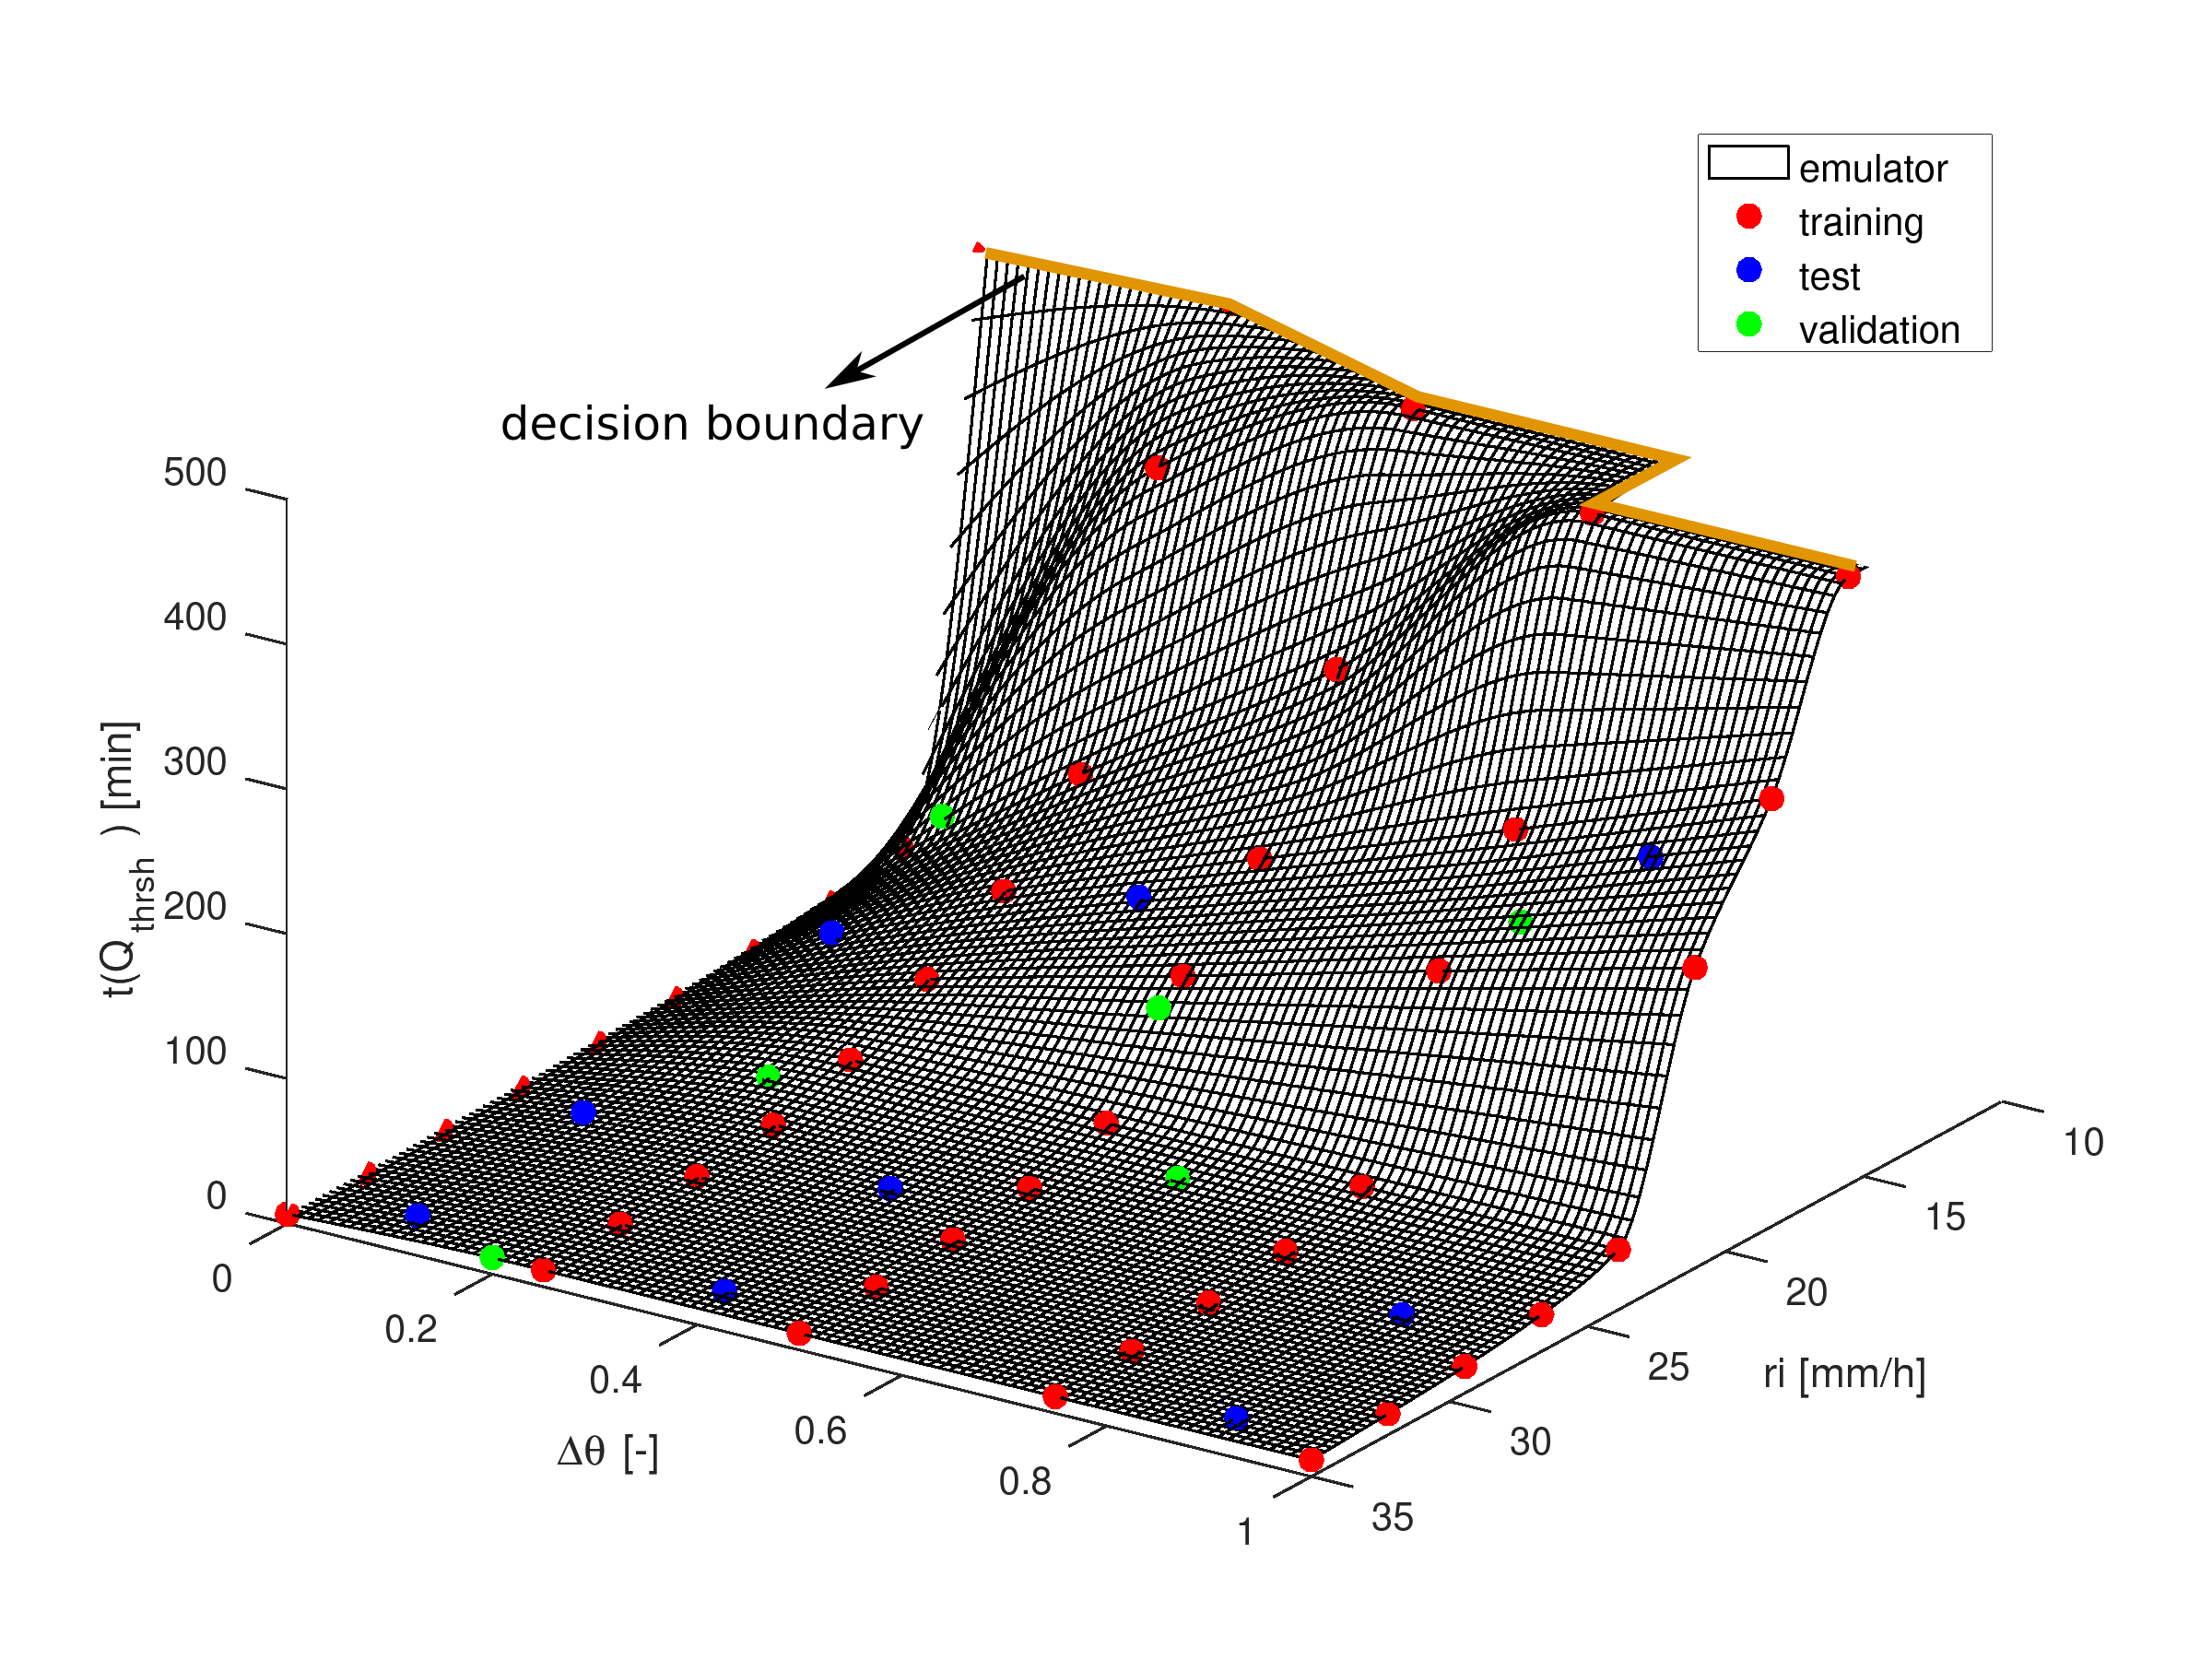
\includegraphics[width=0.4\textwidth]{img/emulator.png}
  \caption{$t_!$ as a function of $I$ and $\Delta\theta$.
  The black mesh shows the prediction of $t_!$ between the sampled points, i.e. our emulator.}
  \label{img:emulator}
\end{figure}

Fig.~\ref{img:emulator} shows the emulator built from the 50 samples of the two varied parameters (\textit{training points}).
Different types of interpolators were tested and their performance was evaluated on the \textit{test points}.
\textit{Validation points} were used in order to have an unbiased assessment of the emulator performance.

For low $I$ and $\Delta\theta$ the chosen $Q_!$ is never reached. This is shown in the figure with the orange frontier: some ($I$, $\Delta\theta$) combinations produce no $t_!$ prediction.



%The hydrographs show different responses depending on the soil initial saturation and the rain intensity which was applied.
%In some cases, in particular by heavy rain and high initial soil saturation values, the appearance of surface runoff is very rapid.
%In other cases this just happens after it has rained for hours or does not happen at all. The emulator we aim to build should be used as an early flood warning system. The variable which it is trying to predict is then the time at which a certain $Q_!$, the maximum discharge for which the various hydraulic structure on the channel downstream of the catchment were dimensioned, is reached. As observable from the hydrographs this time can be very variable depending on the value of $Q_!$ or can never be reached.

\section{Acknowledge}
The authors would like to thank Prof. Peter Molnar and Dr. Jörg Rieckermann for their support and guidance during S. Rusca's master thesis and the writing of this article.
We thank the developers of \citetalias{Octave} and \citetalias{Inkscape} for their excellent software tools, which were used for this article.

Source code is available at \url{bitbucket.org/binello7/master_thesis}.

\paragraph*{Funding} The research leading to these results has received funding from the Eawag's discretionary funding program (project EmuMore \url{kakila.bitbucket.io/emumore}).

\paragraph*{Author contributions}
\textbf{SR} developed the software, carried out simulations, and data analysis.
\textbf{JPC} contributed to the emulator design, data analysis, and supervised SR. All authors contributed to the writing of this manuscript.

\sloppy
\bibliographystyle{unsrtnat}
\bibliography{References}


\end{document}
